%%%%%%%%%%%%%%%%%%%%%%%%%%%%%%%%%%%%%%%%%
% fphw Assignment
% LaTeX Template
% Version 1.0 (27/04/2019)
%
% This template originates from:
% https://www.LaTeXTemplates.com
%
% Authors:
% Class by Felipe Portales-Oliva (f.portales.oliva@gmail.com) with template 
% content and modifications by Vel (vel@LaTeXTemplates.com)
%
% Template (this file) License:
% CC BY-NC-SA 3.0 (http://creativecommons.org/licenses/by-nc-sa/3.0/)
%
%%%%%%%%%%%%%%%%%%%%%%%%%%%%%%%%%%%%%%%%%

%----------------------------------------------------------------------------------------
%	PACKAGES AND OTHER DOCUMENT CONFIGURATIONS
%----------------------------------------------------------------------------------------

\documentclass[
	12pt, % Default font size, values between 10pt-12pt are allowed
	%letterpaper, % Uncomment for US letter paper size
	%spanish, % Uncomment for Spanish
]{fphw}

% Template-specific packages
\usepackage[utf8]{inputenc} % Required for inputting international characters
\usepackage[T1]{fontenc} % Output font encoding for international characters
\usepackage{mathpazo} % Use the Palatino font
\usepackage[dvipsnames]{xcolor}
\usepackage{graphicx} % Required for including images
\usepackage{amsmath}
\usepackage{booktabs} % Required for better horizontal rules in tables
\usepackage{listings} % Required for insertion of code
\usepackage{enumerate} % To modify the enumerate environment
\usepackage{ragged2e}
\usepackage{cancel}
\usepackage{MnSymbol,bbding,pifont}
\usepackage{lscape}
\usepackage{array}
\usepackage{float,graphicx}
\newcolumntype{M}{>{$}c<{$}}
%----------------------------------------------------------------------------------------
%	ASSIGNMENT INFORMATION
%----------------------------------------------------------------------------------------

\title{Assignment \#5} % Assignment title

\author{Luis Alberto Ballado Aradias} % Student name

\date{\today} % Due date

\institute{Centro de Investigación y de Estudios Avanzados del IPN \\ Unidad Tamaulipas} % Institute or school name

\class{Tecnologías Computacionales (Sep - Dec 2022)} % Course or class name

\professor{Dr. Edwin Aldana Bobadilla} % Professor or teacher in charge of the assignment

%----------------------------------------------------------------------------------------

\begin{document}

\maketitle % Output the assignment title, created automatically using the information in the custom commands above

%----------------------------------------------------------------------------------------
%	ASSIGNMENT CONTENT
%----------------------------------------------------------------------------------------

\section*{{\color{Apricot}Memory Allocation}}
%------------------------------------------------

The underlying OS provides some memory to every program that runs and the memory can be divided into two areas.

\begin{itemize}
\item STACK - used to store temporary variables, primitive data types etc. A block in the stack exists for a variable only as long as the variable exists. After that, the block data is erased and it can be used for storing another variable.
\item HEAP - is a special Tree-based data structure in which the tree is a complete binary tree. In heap memory, a physical copy of an object is stored and the reference or address of this copy in the variable of the associated class. Objects that can no longer be referenced are cleaned up by Garbage collector in JAVA language.
\end{itemize}

\begin{figure}[H]
  \centering
  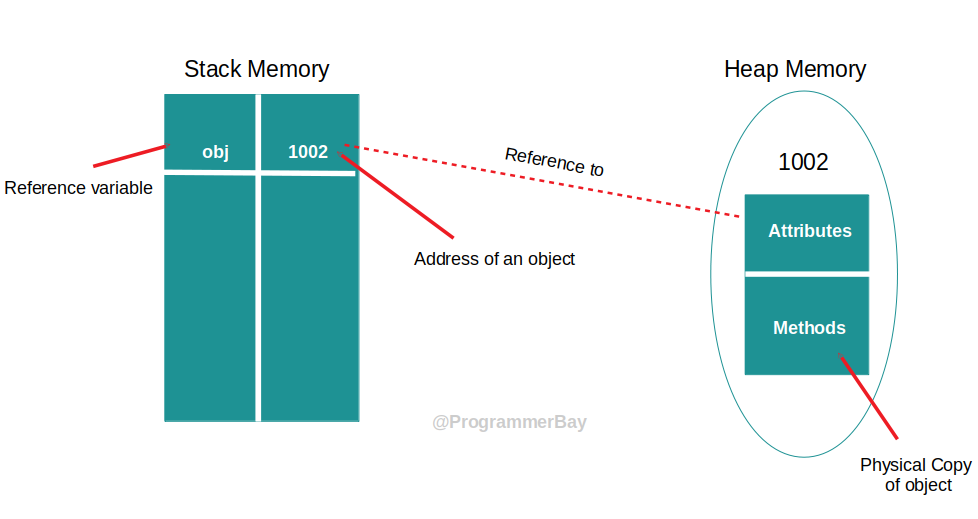
\includegraphics[scale=0.4]{images/object_mem.png}
\end{figure}

In every program there are four entities that need to live on this memory

\begin{itemize}
\item Local Variables - Are the variables that are declared inside a method and they live on the stack, they are temporary and they live on the stack as long as the method is executing, so any current executing method along with its local variables lives on the stack until it is done.
\item Methods - is a procedure associated with a message and an object.
\item Objects - Live on the heap and since we know that the instance variables belong to their respective objects instance variables live inside the object on a heap
\item Instance Variables - is a variable which is declared in a class but outside of constructructors, methods, or blocks. Instance variables are created when an object is created with the use of the keyword 'new' and destroyed when the object is destroyed.
\end{itemize}

For example:\\

A Car Object (\textbf{Car myCar = new Car();}) which has certain instance variables like: gears, wheels, height. So in heap memory the object always has a sufficient amount of memory to contain all its instance variables. \\

Object creation is a two step process \textbf{Declaration} (\textbf{Car myCar}) and \textbf{Instantiation} (\textbf{new Car();}) \\
In my declaration I have declared a reference variable of the type Car. I have used two keywords here the reference variable and the type car. My Car is called a reference variable, because it does not hold the actual object, just a reference or the address of the memory pointing to the actual object, and car is called a type because car is a class.\\

A class is a logical framework that defines the relationship between it is members, so class is nothing but a user-defined data type and of course I can use this data type to create my reference variable instantiation. The new keyword actually creates the object and the memory is allocated to this object for which the reference is assigned to my Car reference variable, there is one thing that is important here. Since the new keyword allocates memory only at runtime, so the memory gets allocated when the program is executing.\\

\textbf{Constructors} \\

\begin{itemize}
\item Every class has a constructor.
\item A compiler provides the default constructor if no constructor is present in the code.
\item Constructor is called during the lifecycle of an object.
\item Constructor provides a fully initialised usable object immediately upon object creation.
  
\end{itemize}

\newpage

There are various types of inheritance, based on paradigm and specific language.

\section*{{\color{Cerulean}Single inheritance}}
%------------------------------------------------
where subclasses inherit the features of one superclass. A class acquires the properties of another class.

\begin{figure}[H]
  \centering
  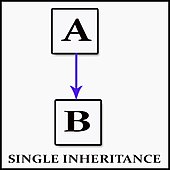
\includegraphics[scale=0.6]{images/170px-Single_Inheritance.jpg}
\end{figure}

Single inheritance enables a derived class to inherit properties and behavior from a single parent class. It allows a derived class to inherit the properties and behavior of a base class, thus enabling code reusability as well as adding new features to the existing code. This makes the code much more elegant and less repetitive. Inheritance is one of the key features of object-oriented programming (OOP). \textbf{Single inheritance} is safer than multiple inheritance if it is approached in the right way. It also enables a derived class to call the parent class implementation for a specific method if this method is overridden in the derived class or the parent class constructor.

\section*{{\color{RoyalPurple}Multiple inheritance}}
%------------------------------------------------

where one class can have more than one superclass and inherit features from all parent classes.

\begin{figure}[H]
  \centering
  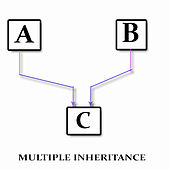
\includegraphics[scale=0.6]{images/170px-Multiple_Inheritance.jpg}
\end{figure}

Multiple Inheritance is a feature of C++ where a class can inherit from more than one classes.  The constructors of inherited classes are called in the same order in which they are inherited. For example, in the following program, B’s constructor is called before A’s constructor. A class can be derived from more than one base class. (i.e. A CHILD class is derived from FATHER and MOTHER class.) \\

Unlike some other popular object oriented programming languages like C++, java doesn’t provide support for multiple inheritance in classes. Java doesn’t support multiple inheritances in classes because it can lead to diamond problem and rather than providing some complex way to solve it, there are better ways through which we can achieve the same result as multiple inheritances.

\end{document}
